\documentclass{article}
\usepackage{pgfplots}
\usepackage{caption}

\begin{document}

\begin{figure}[h]
    \centering
    \begin{tikzpicture}
        \begin{axis}[
            title={Material Deformations},
            xlabel={Strain (dimensionless)},
            ylabel={Stress (dimensionless)},
            xmin=0, xmax=1,
            ymin=0, ymax=1,
            xtick={0,0.2,...,1},
            ytick={0,0.2,...,1},
            grid=major,
            legend pos=north west,
            width=\textwidth,
            height=0.8\textheight,
            legend style={nodes={scale=0.7, transform shape}},
            ]
            \addplot[red, thick] coordinates {(0,0) (0.5,0.5) (1,1)};
            \addlegendentry{Unloaded}
            
            \addplot[blue, thick] coordinates {(0,0) (0.5,0.5) (1,1)};
            \addlegendentry{Tension}
            
            \addplot[green, thick] coordinates {(0,0) (0.5,0.5) (1,1)};
            \addlegendentry{Bending}
            
            \addplot[orange, thick] coordinates {(0,0) (0.5,0.5) (1,1)};
            \addlegendentry{Shear}
        \end{axis}
    \end{tikzpicture}
    \captionof{figure}{Material Deformations: Unloaded, Tension, Bending, Shear}
    \label{fig:material_deformations}
\end{figure}

\begin{figure}[h]
    \centering
    \begin{tikzpicture}
        \begin{axis}[
            title={Material Deformations},
            xlabel={Strain (dimensionless)},
            ylabel={Stress (dimensionless)},
            xmin=0, xmax=1,
            ymin=0, ymax=1,
            xtick={0,0.2,...,1},
            ytick={0,0.2,...,1},
            grid=major,
            legend pos=north west,
            width=\textwidth,
            height=0.8\textheight,
            legend style={nodes={scale=0.7, transform shape}},
            ]
            \addplot[red, thick] coordinates {(0,0) (0.5,0.5) (1,1)};
            \addlegendentry{Unloaded}
            
            \addplot[blue, thick] coordinates {(0,0) (0.5,0.5) (1,1)};
            \addlegendentry{Tension}
            
            \addplot[green, thick] coordinates {(0,0) (0.5,0.5) (1,1)};
            \addlegendentry{Bending}
            
            \addplot[orange, thick] coordinates {(0,0) (0.5,0.5) (1,1)};
            \addlegendentry{Shear}
        \end{axis}
    \end{tikzpicture}
    \captionof{figure}{Material Deformations: Unloaded, Tension, Bending, Shear}
    \label{fig:material_deformations_2}
\end{figure}

% Continue adding similar figures as needed

\end{document}